\documentclass[11pt,a4paper]{report}
\usepackage[textwidth=37em,vmargin=30mm]{geometry}
\usepackage{calc,xunicode,amsmath,amssymb,paralist,enumitem,tabu,booktabs,datetime2,xeCJK,xeCJKfntef,listings}
\usepackage{tocloft,fancyhdr,tcolorbox,xcolor,graphicx,eso-pic,xltxtra,xelatexemoji}

\newcommand{\envyear}[0]{2025}
\newcommand{\envdatestr}[0]{2025-04-04}
\newcommand{\envfinaldir}[0]{webdb/2025/20250404/final}

\usepackage[hidelinks]{hyperref}
\hypersetup{
    colorlinks=false,
    pdfpagemode=FullScreen,
    pdftitle={Web Digest - \envdatestr}
}

\setlength{\cftbeforechapskip}{10pt}
\renewcommand{\cftchapfont}{\rmfamily\bfseries\large\raggedright}
\setlength{\cftbeforesecskip}{2pt}
\renewcommand{\cftsecfont}{\sffamily\small\raggedright}

\setdefaultleftmargin{2em}{2em}{1em}{1em}{1em}{1em}

\usepackage{xeCJK,xeCJKfntef}
\xeCJKsetup{PunctStyle=plain,RubberPunctSkip=false,CJKglue=\strut\hskip 0pt plus 0.1em minus 0.05em,CJKecglue=\strut\hskip 0.22em plus 0.2em}
\XeTeXlinebreaklocale "zh"
\XeTeXlinebreakskip = 0pt


\setmainfont{Brygada 1918}
\setromanfont{Brygada 1918}
\setsansfont{IBM Plex Sans}
\setmonofont{JetBrains Mono NL}
\setCJKmainfont{Noto Serif CJK SC}
\setCJKromanfont{Noto Serif CJK SC}
\setCJKsansfont{Noto Sans CJK SC}
\setCJKmonofont{Noto Sans CJK SC}

\setlength{\parindent}{0pt}
\setlength{\parskip}{8pt}
\linespread{1.15}

\lstset{
	basicstyle=\ttfamily\footnotesize,
	numbersep=5pt,
	backgroundcolor=\color{black!5},
	showspaces=false,
	showstringspaces=false,
	showtabs=false,
	tabsize=2,
	captionpos=b,
	breaklines=true,
	breakatwhitespace=true,
	breakautoindent=true,
	linewidth=\textwidth
}






\newcommand{\coverpic}[2]{
    % argv: itemurl, authorname
    Cover photo by #2~~(\href{#1}{#1})
}
\newcommand{\makeheader}[0]{
    \begin{titlepage}
        % \newgeometry{hmargin=15mm,tmargin=21mm,bmargin=12mm}
        \begin{center}
            
            \rmfamily\scshape
            \fontspec{BaskervilleF}
            \fontspec{Old Standard}
            \fontsize{59pt}{70pt}\selectfont
            WEB\hfill DIGEST
            
            \vfill
            % \vskip 30pt
            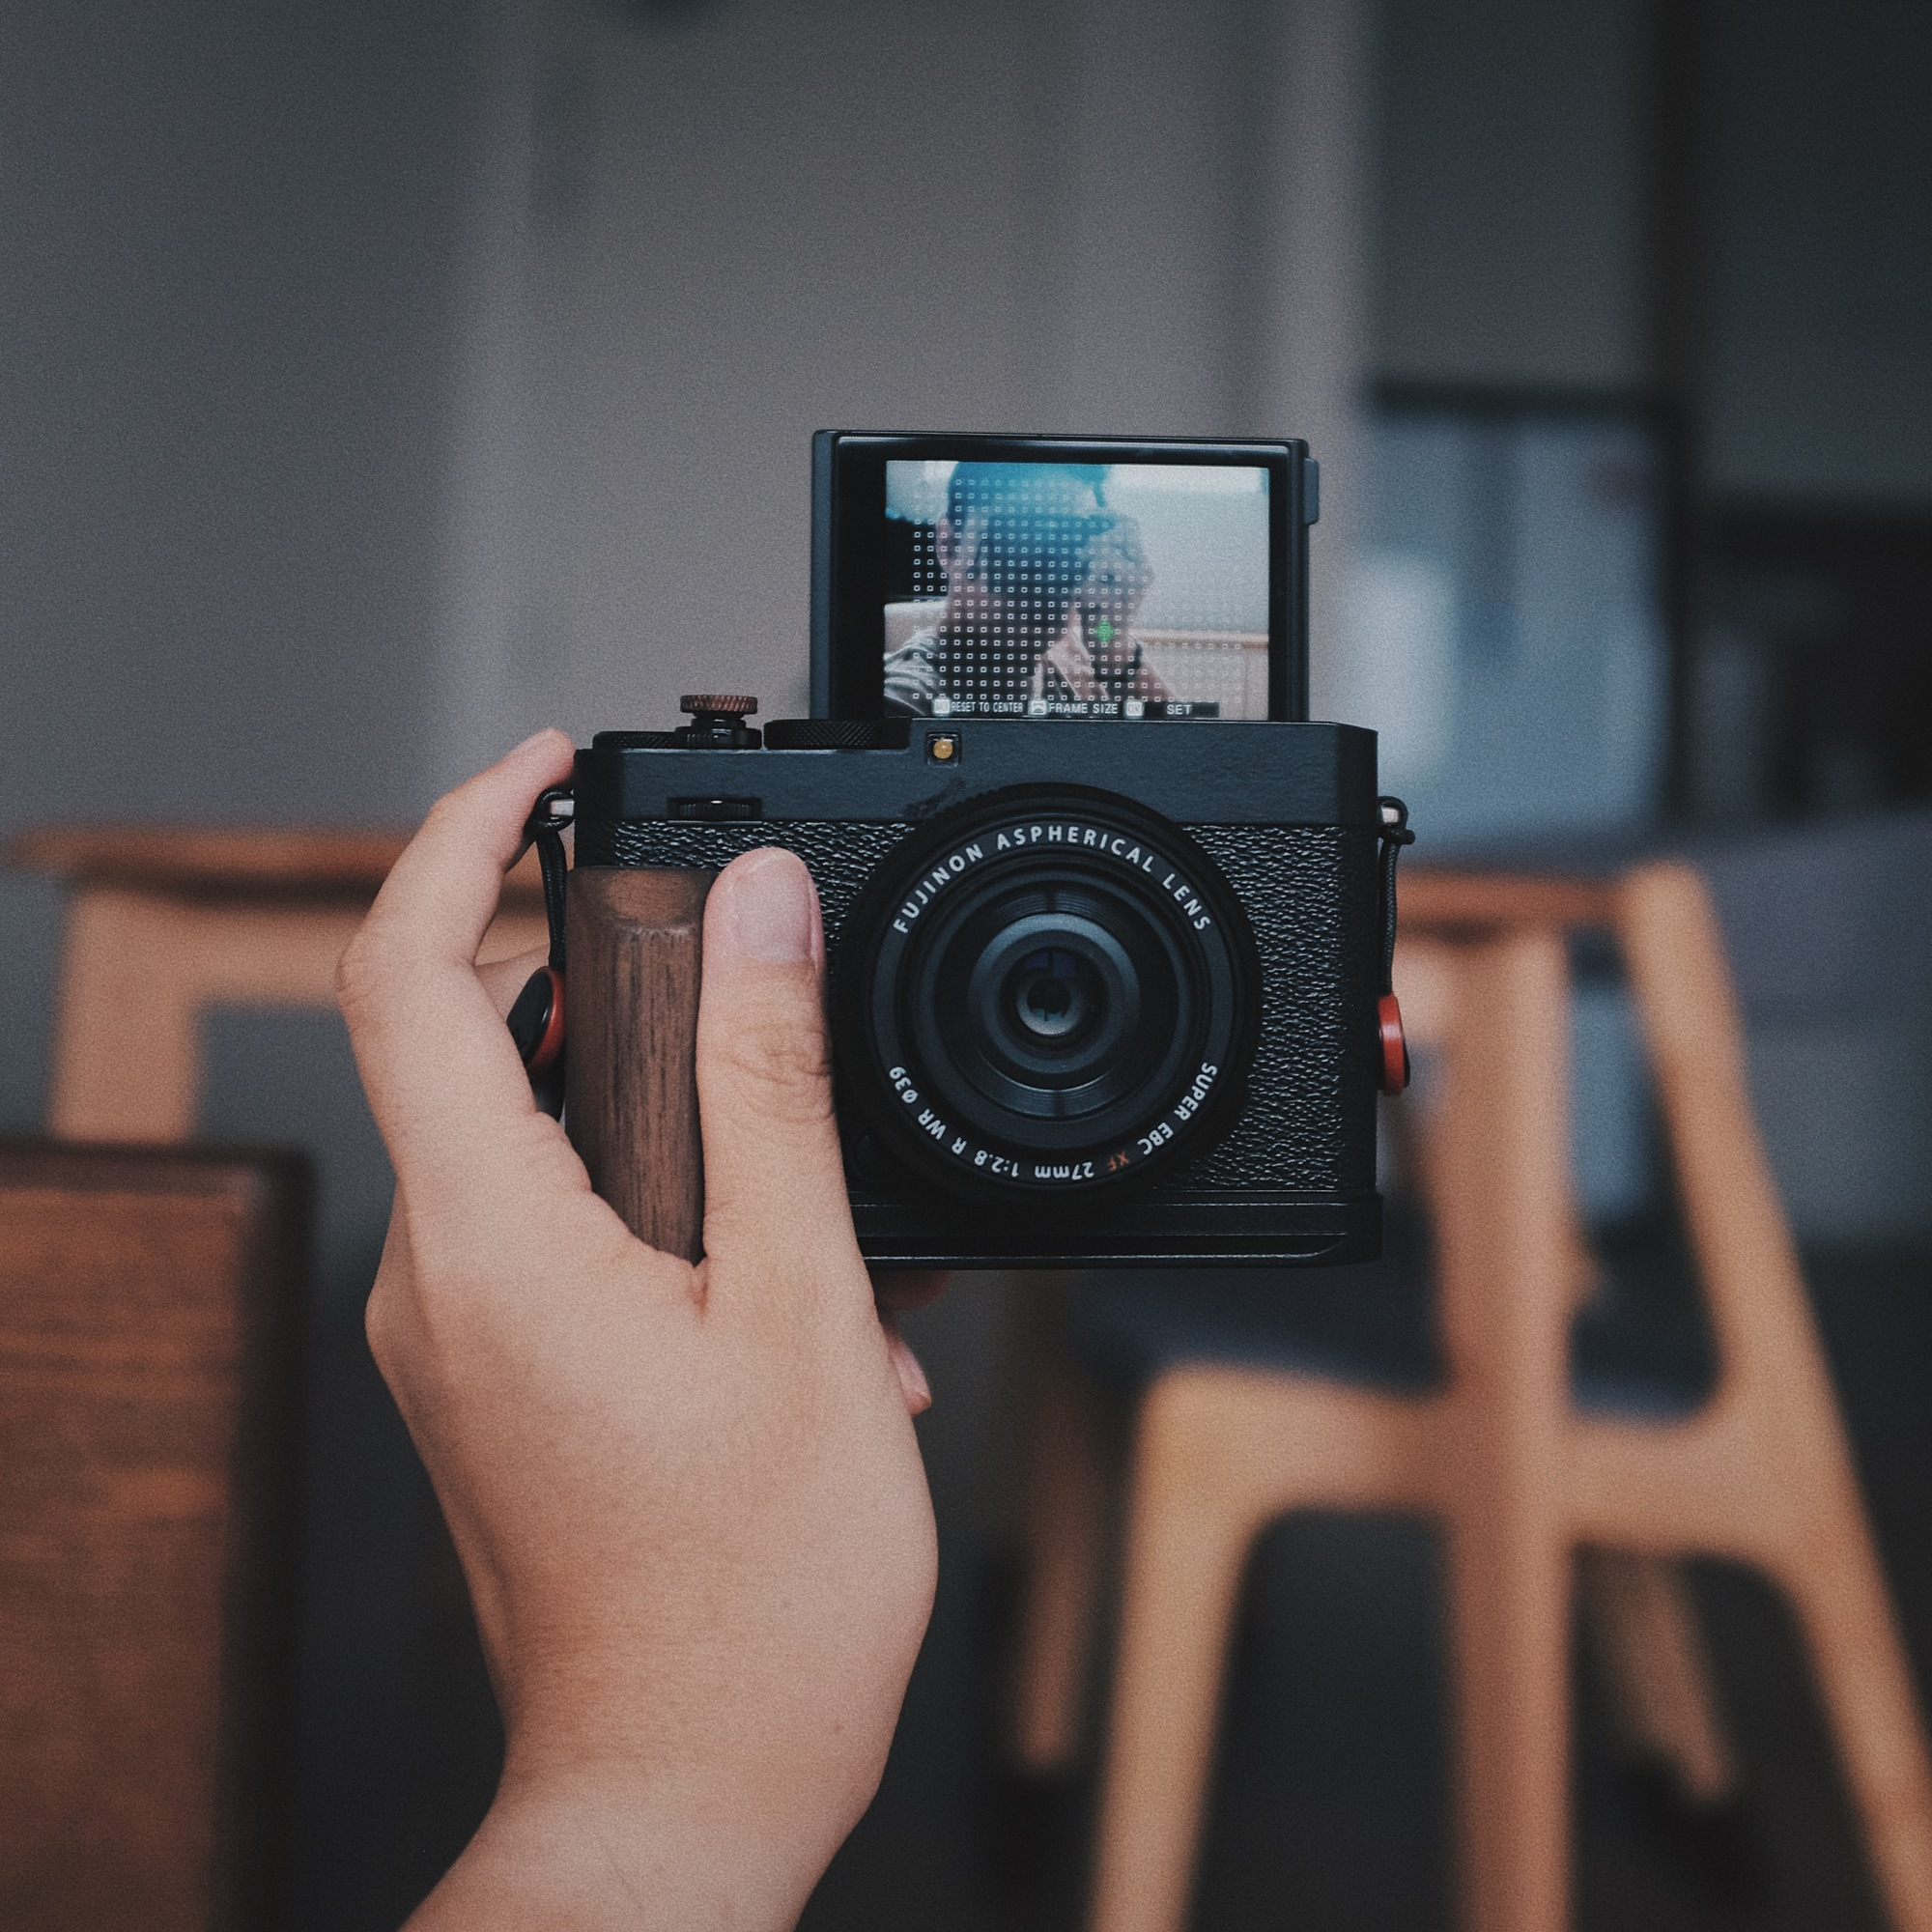
\includegraphics[width=\linewidth]{\envfinaldir/coverpic-prod.jpg}\par
            % \vskip 30pt
            \vfill

            \normalsize\rmfamily\scshape
            \copyright{} The Web Digest Project \hfill\large \envdatestr
        \end{center}
    \end{titlepage}
    % \restoregeometry
}
\newcommand{\simplehref}[1]{%
    \textcolor{blue!80!green}{\href{#1}{#1}}%
}
\renewcommand{\contentsname}{\center\Huge\sffamily\bfseries Contents\par\vskip 20pt}
\newcounter{ipartcounter}
\setcounter{ipartcounter}{0}
\newcommand{\ipart}[1]{
    % \vskip 20pt
    \clearpage
    \stepcounter{ipartcounter}
    \phantomsection
    \addcontentsline{toc}{chapter}{#1}
    % \begin{center}
    %     \Huge
    %     \sffamily\bfseries
    %     #1
    % \end{center}
    % \vskip 20pt plus 7pt
}
\newcounter{ichaptercounter}
\setcounter{ichaptercounter}{0}
\newcommand{\ichapter}[1]{
    % \vskip 20pt
    \clearpage
    \stepcounter{ichaptercounter}
    \phantomsection
    \addcontentsline{toc}{section}{\numberline{\arabic{ichaptercounter}}#1}
    \begin{center}
        \Huge
        \sffamily\bfseries
        #1
    \end{center}
    \vskip 20pt plus 7pt
}
\newcommand{\entrytitlefont}[1]{\subsection*{\raggedright\Large\sffamily\bfseries#1}}
\newcommand{\entryitemGeneric}[2]{
    % argv: title, url
    \parbox{\linewidth}{
        \entrytitlefont{#1}\par\vskip 5pt
        \footnotesize\ttfamily\mdseries
        \simplehref{#2}
    }\vskip 11pt plus 11pt minus 1pt
}
\newcommand{\entryitemGithub}[3]{
    % argv: title, url, desc
    \parbox{\linewidth}{
        \entrytitlefont{#1}\par\vskip 5pt
        \footnotesize\ttfamily\mdseries
        \simplehref{#2}\par\vskip 5pt
        \small\rmfamily\mdseries#3
    }\vskip 11pt plus 11pt minus 1pt
}
\newcommand{\entryitemAp}[3]{
    % argv: title, url, desc
    \parbox{\linewidth}{
        \entrytitlefont{#1}\par\vskip 5pt
        \footnotesize\ttfamily\mdseries
        \simplehref{#2}\par\vskip 5pt
        \small\rmfamily\mdseries#3
    }\vskip 11pt plus 11pt minus 1pt
}
\newcommand{\entryitemHackernews}[3]{
    % argv: title, hnurl, rawurl
    % \parbox{\linewidth}{
    %     \entrytitlefont{#1}\par\vskip 5pt
    %     \footnotesize\ttfamily\mdseries
    %     \simplehref{#3}\par
    %     \textcolor{black!50}{\href{#2}{#2}}
    % }\vskip 11pt plus 11pt minus 1pt
    \begin{minipage}{\linewidth}
            \entrytitlefont{#1}\par\vskip 5pt
            \footnotesize\ttfamily\mdseries
            \simplehref{#3}\par
            \textcolor{black!50}{\href{#2}{#2}}
    \end{minipage}\par\vskip 11pt plus 11pt minus 1pt
}







\begin{document}

\makeheader

\tableofcontents\clearpage




\ipart{Developers}
\ichapter{Hacker News}
\entryitemTwoLinks{An image of an archeologist adventurer who wears a hat and uses a bullwhip}{https://news.ycombinator.com/item?id=43573156}{https://theaiunderwriter.substack.com/p/an-image-of-an-archeologist-adventurer}

\entryitemTwoLinks{Reasoning models don't always say what they think}{https://news.ycombinator.com/item?id=43572374}{https://www.anthropic.com/research/reasoning-models-dont-say-think}

\entryitemTwoLinks{AI 2027}{https://news.ycombinator.com/item?id=43571851}{https://ai-2027.com/}

\entryitemTwoLinks{Curl-impersonate: Special build of curl that can impersonate the major browsers}{https://news.ycombinator.com/item?id=43571099}{https://github.com/lwthiker/curl-impersonate}

\entryitemTwoLinks{AnimeJs v4 Is Here}{https://news.ycombinator.com/item?id=43570533}{https://animejs.com/}

\entryitemTwoLinks{Overengineered Anchor Links}{https://news.ycombinator.com/item?id=43570324}{https://thirty-five.com/overengineered-anchoring}

\entryitemTwoLinks{Show HN: OpenNutrition – A free, public nutrition database}{https://news.ycombinator.com/item?id=43569190}{https://www.opennutrition.app/search}

\entryitemTwoLinks{Hackers stole billions in crypto to keep North Korea's regime afloat}{https://news.ycombinator.com/item?id=43569009}{https://www.wsj.com/world/asia/north-korea-cryptocurrency-580d7d3f}

\entryitemTwoLinks{A university president makes a case against cowardice}{https://news.ycombinator.com/item?id=43568655}{https://www.newyorker.com/news/q-and-a/a-university-president-makes-a-case-against-cowardice}

\entryitemTwoLinks{InitWare, a portable systemd fork running on BSDs and Linux}{https://news.ycombinator.com/item?id=43568503}{https://github.com/InitWare/InitWare}

\entryitemTwoLinks{The Steam Deck is software-freedom friendly}{https://news.ycombinator.com/item?id=43567923}{https://isomorphism.xyz/blog/2024/steam-deck/}

\entryitemTwoLinks{DIY Synths Database}{https://news.ycombinator.com/item?id=43564890}{https://diy-synths.snnkv.com/}

\entryitemTwoLinks{Dijkstra On the foolishness of "natural language programming"}{https://news.ycombinator.com/item?id=43564386}{https://www.cs.utexas.edu/~EWD/transcriptions/EWD06xx/EWD667.html}

\entryitemTwoLinks{I maintain a 17 year old ThinkPad}{https://news.ycombinator.com/item?id=43564111}{https://pilledtexts.com/why-i-use-a-17-year-old-thinkpad/}

\entryitemTwoLinks{Tech companies are telling immigrant employees on visas not to leave the U.S.}{https://news.ycombinator.com/item?id=43563918}{https://www.washingtonpost.com/technology/2025/03/31/immigration-h1b-fear-siliconvalley/}

\entryitemTwoLinks{The reality of working in tech: We're not hired to write code (2023)}{https://news.ycombinator.com/item?id=43563533}{https://idiallo.com/blog/code-for-hire}

\entryitemTwoLinks{An open source, self-hosted implementation of the Tailscale control server}{https://news.ycombinator.com/item?id=43563396}{https://github.com/juanfont/headscale}

\entryitemTwoLinks{Web Server for AoE 1, 2 and 3 DE supporting LAN multiplayer 100\% offline}{https://news.ycombinator.com/item?id=43562860}{https://github.com/luskaner/ageLANServer}

\entryitemTwoLinks{Multi-Token Attention}{https://news.ycombinator.com/item?id=43562384}{https://arxiv.org/abs/2504.00927}

\entryitemTwoLinks{Are people bad at their jobs or are the jobs just bad?}{https://news.ycombinator.com/item?id=43562119}{https://annehelen.substack.com/p/are-people-bad-at-their-jobsor-are}\ichapter{Phoronix}
\entryitemGeneric{\hskip 0pt{}AMD's AOMP 21.0 Switches To New Fortran Compiler, Delivers More Performance}{https://www.phoronix.com/news/AOMP-21.0-0-Compiler}

\entryitemGeneric{\hskip 0pt{}OpenCL 3.0.18 Published With New Extensions \& Other Updates}{https://www.phoronix.com/news/OpenCL-3.0.18}

\entryitemGeneric{\hskip 0pt{}AMD Ryzen 9 9900X3D Impact Of The 3D V-Cache Optimizer Linux Driver}{https://www.phoronix.com/review/amd-9900x3d-3d-v-cache}

\entryitemGeneric{\hskip 0pt{}Intel Updates Linux Patches For Adaptive Sharpness Property, Xe VRAM Self Refresh}{https://www.phoronix.com/news/Intel-Adaptive-Sharpness-VRSR}

\entryitemGeneric{\hskip 0pt{}Linux 6.15's New "hugetlb\_alloc\_threads" Option Can Help Speed-Up Boot Times}{https://www.phoronix.com/news/Linux-6.15-MM}

\entryitemGeneric{\hskip 0pt{}Intel Patches Finally Exposing NPU Frequency Under Linux}{https://www.phoronix.com/news/Intel-Linux-NPU-Frequency-Patch}

\entryitemGeneric{\hskip 0pt{}Linux 6.15 Brings Improvements For Five Decade Old GPIB Bus}{https://www.phoronix.com/news/Linux-6.15-Staging}

\entryitemGeneric{\hskip 0pt{}Linux 6.15 Device Mapper Brings Inline Crypto Passthrough For DM-Stripe}{https://www.phoronix.com/news/Linux-6.15-DM}

\entryitemGeneric{\hskip 0pt{}Rust 1.86 Released With Trait Upcasting, Deprecates i586-PC-Windows-MSVC}{https://www.phoronix.com/news/Rust-1.86-Released}\ichapter{Dribbble}
\entryitemGeneric{\hskip 0pt{}Ship Logo Design - Boat, Shield, Star, Waves}{https://dribbble.com/shots/25854151-Ship-Logo-Design-Boat-Shield-Star-Waves}

\entryitemGeneric{\hskip 0pt{}Interactive Speed Slider}{https://dribbble.com/shots/25851176-Interactive-Speed-Slider}

\entryitemGeneric{\hskip 0pt{}Abstract}{https://dribbble.com/shots/25853030-Abstract}

\entryitemGeneric{\hskip 0pt{}Croc logo}{https://dribbble.com/shots/25852607-Croc-logo}

\entryitemGeneric{\hskip 0pt{}Logo Design Selection Q1 2025}{https://dribbble.com/shots/25852275-Logo-Design-Selection-Q1-2025}

\entryitemGeneric{\hskip 0pt{}Cloud Lightning}{https://dribbble.com/shots/25852815-Cloud-Lightning}

\entryitemGeneric{\hskip 0pt{}ef monogram}{https://dribbble.com/shots/25847206-ef-monogram}

\entryitemGeneric{\hskip 0pt{}Outrigger Marketing Logo}{https://dribbble.com/shots/25848681-Outrigger-Marketing-Logo}

\entryitemGeneric{\hskip 0pt{}Helpfull - Logo Redesign}{https://dribbble.com/shots/25847828-Helpfull-Logo-Redesign}

\entryitemGeneric{\hskip 0pt{}Letter G set}{https://dribbble.com/shots/25845864-Letter-G-set}

\entryitemGeneric{\hskip 0pt{}Wayflow Logo Design - Letter W, Waves, Flow}{https://dribbble.com/shots/25847473-Wayflow-Logo-Design-Letter-W-Waves-Flow}

\entryitemGeneric{\hskip 0pt{}Vínföng Final Wordmark}{https://dribbble.com/shots/25848505-V-nf-ng-Final-Wordmark}

\entryitemGeneric{\hskip 0pt{}Prana Symbol}{https://dribbble.com/shots/25847656-Prana-Symbol}

\entryitemGeneric{\hskip 0pt{}Let down your hair}{https://dribbble.com/shots/25844844-Let-down-your-hair}

\entryitemGeneric{\hskip 0pt{}Chat GPT 4 Branding Concept}{https://dribbble.com/shots/25844194-Chat-GPT-4-Branding-Concept}

\entryitemGeneric{\hskip 0pt{}Sustainable contribution selector: percentage picker}{https://dribbble.com/shots/25843734-Sustainable-contribution-selector-percentage-picker}

\entryitemGeneric{\hskip 0pt{}FG}{https://dribbble.com/shots/25842733-FG}

\entryitemGeneric{\hskip 0pt{}Kovre Winery Logo Exploration}{https://dribbble.com/shots/25844706-Kovre-Winery-Logo-Exploration}

\entryitemGeneric{\hskip 0pt{}Cloud Paper}{https://dribbble.com/shots/25844908-Cloud-Paper}

\entryitemGeneric{\hskip 0pt{}Core 2.0 – Dashboard Builder - Mobile view}{https://dribbble.com/shots/25844403-Core-2-0-Dashboard-Builder-Mobile-view}

\entryitemGeneric{\hskip 0pt{}Crypto Portfolio Dashboard}{https://dribbble.com/shots/25841268-Crypto-Portfolio-Dashboard}

\entryitemGeneric{\hskip 0pt{}Finergy app UI Kit on UI8}{https://dribbble.com/shots/25837473-Finergy-app-UI-Kit-on-UI8}

\entryitemGeneric{\hskip 0pt{}Weylix Logo Design - W Letter Monogram, Wave}{https://dribbble.com/shots/25834720-Weylix-Logo-Design-W-Letter-Monogram-Wave}

\entryitemGeneric{\hskip 0pt{}BB}{https://dribbble.com/shots/25834486-BB}


\ipart{Developers~~~~(zh-Hans)}
\ichapter{Solidot}
\entryitemGeneric{\hskip 0pt{}朝鲜黑客如何窃取数以十亿美元的加密货币}{https://www.solidot.org/story?sid=80967}

\entryitemGeneric{\hskip 0pt{}美国 34 家比特币矿场的耗电量超过洛杉矶}{https://www.solidot.org/story?sid=80966}

\entryitemGeneric{\hskip 0pt{}小行星 2024 YR4 撞击月球概率上调至 3.8\%}{https://www.solidot.org/story?sid=80965}

\entryitemGeneric{\hskip 0pt{}盖茨以 PDF 形式发布了 Altair BASIC 源代码}{https://www.solidot.org/story?sid=80964}

\entryitemGeneric{\hskip 0pt{}美国富人的寿命低于欧洲富人}{https://www.solidot.org/story?sid=80963}

\entryitemGeneric{\hskip 0pt{}部分音乐享受能力或来自遗传}{https://www.solidot.org/story?sid=80962}

\entryitemGeneric{\hskip 0pt{}微软 CTO 预测五年内 95\% 的代码由 AI 生成}{https://www.solidot.org/story?sid=80961}

\entryitemGeneric{\hskip 0pt{}雄性果蝇饮酒能增加对雌性的吸引力}{https://www.solidot.org/story?sid=80960}

\entryitemGeneric{\hskip 0pt{}PorteuX 2.0 释出}{https://www.solidot.org/story?sid=80959}

\entryitemGeneric{\hskip 0pt{}维基基金会称 AI 爬虫导致带宽消耗增加五成}{https://www.solidot.org/story?sid=80958}

\entryitemGeneric{\hskip 0pt{}任天堂将第一方游戏售价提高到 70/80 美元}{https://www.solidot.org/story?sid=80957}

\entryitemGeneric{\hskip 0pt{}丢弃的锂离子电池引发火灾}{https://www.solidot.org/story?sid=80956}

\entryitemGeneric{\hskip 0pt{}贝莱德 CEO 称比特币可能取代美元成为全世界的储备货币}{https://www.solidot.org/story?sid=80955}

\entryitemGeneric{\hskip 0pt{}Rockbox 4.0 释出}{https://www.solidot.org/story?sid=80954}

\entryitemGeneric{\hskip 0pt{}Switch 2 将于 6 月 5 日上市,起售价 450 美元}{https://www.solidot.org/story?sid=80953}

\entryitemGeneric{\hskip 0pt{}Steam 平台的 Linux 份额达到 2.33\%}{https://www.solidot.org/story?sid=80952}

\entryitemGeneric{\hskip 0pt{}到本世纪末如果全球气温上升 3°C 全世界四成经济可能会被抹掉}{https://www.solidot.org/story?sid=80951}

\entryitemGeneric{\hskip 0pt{}年轻男性泡冷水澡或有助于身体健康}{https://www.solidot.org/story?sid=80950}

\entryitemGeneric{\hskip 0pt{}每周三天间歇性禁食减肥效果显著}{https://www.solidot.org/story?sid=80949}

\entryitemGeneric{\hskip 0pt{}OpenAI 被指控未经授权使用 O'Reilly 书籍训练 GPT-4o}{https://www.solidot.org/story?sid=80948}\ichapter{V2EX}
\entryitemGeneric{\hskip 0pt{}[扬州] 今年扬州琼花开花时间大约几号}{https://www.v2ex.com/t/1123247}

\entryitemGeneric{\hskip 0pt{}[Apple] 国行 iPhone 17 系列接入 esim}{https://www.v2ex.com/t/1123246}

\entryitemGeneric{\hskip 0pt{}[酷工作] [北京/全职] 后端开发工程师}{https://www.v2ex.com/t/1123244}

\entryitemGeneric{\hskip 0pt{}[程序员] 有没有免费的 OCR API?自己服务器能部署的开源软件也行}{https://www.v2ex.com/t/1123243}

\entryitemGeneric{\hskip 0pt{}[Apple] iOS 18.4 设置显示 BUG}{https://www.v2ex.com/t/1123242}

\entryitemGeneric{\hskip 0pt{}[程序员] 旧笔记本用途 拯救者 y7000p 2020}{https://www.v2ex.com/t/1123240}

\entryitemGeneric{\hskip 0pt{}[电动汽车] 如果小米 NOA 要为事故担责,那么恭喜雷布斯了,中国第一个 L3 智驾车企!}{https://www.v2ex.com/t/1123237}

\entryitemGeneric{\hskip 0pt{}[程序员] 付费爬外网}{https://www.v2ex.com/t/1123236}

\entryitemGeneric{\hskip 0pt{}[问与答] 大佬们的自创的桌面端 app 去哪里推广?}{https://www.v2ex.com/t/1123235}

\entryitemGeneric{\hskip 0pt{}[macOS] 系统安装在外置硬盘的 Mac Mini M4 有成功升级到 15.4 的吗}{https://www.v2ex.com/t/1123234}

\entryitemGeneric{\hskip 0pt{}[职场话题] 自媒体创业笔记:两个爆火短视频连续被限流,不愧是逼格最高的短视频平台-小红书}{https://www.v2ex.com/t/1123233}

\entryitemGeneric{\hskip 0pt{}[程序员] 有会写 solidity 的吗?发个外包}{https://www.v2ex.com/t/1123232}

\entryitemGeneric{\hskip 0pt{}[iPhone] 在电脑上的钥匙链清理工具,无需越狱}{https://www.v2ex.com/t/1123231}

\entryitemGeneric{\hskip 0pt{}[问与答] 中科院自动化研究所工作体验怎么样?}{https://www.v2ex.com/t/1123230}

\entryitemGeneric{\hskip 0pt{}[问与答] 大家的 Gemini 2.5 Pro 卡么?}{https://www.v2ex.com/t/1123229}

\entryitemGeneric{\hskip 0pt{}[Twitter] 发 x 的时候,输入网址的预览卡片多久更新一次的}{https://www.v2ex.com/t/1123228}

\entryitemGeneric{\hskip 0pt{}[分享创造] 做了一个在线 AI 文字编辑器,可以让 AI 批量增删查改,聚类分析,抽取数据,找出遗漏等各种编辑工作}{https://www.v2ex.com/t/1123227}

\entryitemGeneric{\hskip 0pt{}[宽带症候群] 新加坡家宽送的路由器竟然是 BE18000....}{https://www.v2ex.com/t/1123226}

\entryitemGeneric{\hskip 0pt{}[问与答] 相对成本下的服务器数据增量备份与云同步的请教}{https://www.v2ex.com/t/1123224}

\entryitemGeneric{\hskip 0pt{}[macOS] 有人试过 DEVONthink 4.0 beta 了吗?}{https://www.v2ex.com/t/1123223}

\entryitemGeneric{\hskip 0pt{}[Windows] 有办法彻底关掉 win11 自带的剪切板工具吗}{https://www.v2ex.com/t/1123222}

\entryitemGeneric{\hskip 0pt{}[Android] 华为应用市场是如何在不给读取应用列表权限的情况下,获取到要更新的应用的?}{https://www.v2ex.com/t/1123221}

\entryitemGeneric{\hskip 0pt{}[宽带症候群] 陕西电信对 v6 也进行限速了}{https://www.v2ex.com/t/1123219}

\entryitemGeneric{\hskip 0pt{}[问与答] pip 怎么解决两个第三方依赖库的版本冲突的问题}{https://www.v2ex.com/t/1123218}

\entryitemGeneric{\hskip 0pt{}[问与答] 想入一个扫地机器人, V 友们有推荐吗}{https://www.v2ex.com/t/1123217}

\entryitemGeneric{\hskip 0pt{}[问与答] 除了闲鱼,你们还会在什么地方卖二手闲置}{https://www.v2ex.com/t/1123216}

\entryitemGeneric{\hskip 0pt{}[程序员] 求助, Picviewer CE+ 中的一个功能会导致 Alt+D 切换到浏览器地址栏时常失灵}{https://www.v2ex.com/t/1123215}

\entryitemGeneric{\hskip 0pt{}[问与答] 远程工作的程序员应该如何更多地与他人接触,保持正常的社交活动?}{https://www.v2ex.com/t/1123213}

\entryitemGeneric{\hskip 0pt{}[问与答] 在三维欧式空间中,最多能放置多少条直线,才能确保任意选取的三条直线均不共面?}{https://www.v2ex.com/t/1123212}

\entryitemGeneric{\hskip 0pt{}[程序员] [疑惑]-2025-04-03 连续地址分配}{https://www.v2ex.com/t/1123211}

\entryitemGeneric{\hskip 0pt{}[生活] 身边有码农喜欢纹身的吗?纹身有什么暗示么}{https://www.v2ex.com/t/1123210}

\entryitemGeneric{\hskip 0pt{}[投资] 现在不光有缅 A,还有缅纳?}{https://www.v2ex.com/t/1123209}

\entryitemGeneric{\hskip 0pt{}[Apple] 有没有办法能阻止 parsec 自动创建虚拟屏幕吗}{https://www.v2ex.com/t/1123207}

\entryitemGeneric{\hskip 0pt{}[职场话题] 公司要求在清明节期间退还前年年终奖}{https://www.v2ex.com/t/1123206}

\entryitemGeneric{\hskip 0pt{}[程序员] [求助]宿主机无法 ping 通 docker 的 ubuntu 容器}{https://www.v2ex.com/t/1123205}

\entryitemGeneric{\hskip 0pt{}[问与答] Windows 上微信滚动太慢了,有没有办法优化}{https://www.v2ex.com/t/1123204}

\entryitemGeneric{\hskip 0pt{}[问与答] 库巴亚西😭}{https://www.v2ex.com/t/1123203}

\entryitemGeneric{\hskip 0pt{}[问与答] 技术角度,法律角度,宣传角度,这三个视角下的智驾完全不是一回事}{https://www.v2ex.com/t/1123202}

\entryitemGeneric{\hskip 0pt{}[分享创造] 再谈 Backlink Dirs}{https://www.v2ex.com/t/1123201}

\entryitemGeneric{\hskip 0pt{}[分享创造] [新作品] 烽翎 - 跨系统同步剪贴板与管理云端文件}{https://www.v2ex.com/t/1123200}

\entryitemGeneric{\hskip 0pt{}[分享创造] 记 QUIC 的折腾记录}{https://www.v2ex.com/t/1123199}

\entryitemGeneric{\hskip 0pt{}[程序员] 如何将 MCP 运用到 Agentic RAG 系统}{https://www.v2ex.com/t/1123198}

\entryitemGeneric{\hskip 0pt{}[程序员] 帮推荐一下 iOS 平台上接受消息提醒的 app,比如 NotifyMe}{https://www.v2ex.com/t/1123196}

\entryitemGeneric{\hskip 0pt{}[硬件] 蓝牙通断器功耗一般多少?}{https://www.v2ex.com/t/1123195}

\entryitemGeneric{\hskip 0pt{}[macOS] macos 15.4 关闭 SIP 后还是无法开启 swap}{https://www.v2ex.com/t/1123194}

\entryitemGeneric{\hskip 0pt{}[奇思妙想] deepseek 确实量大管饱,价格也是非常便宜,这次确实赢了。}{https://www.v2ex.com/t/1123193}

\entryitemGeneric{\hskip 0pt{}[健康] 用电脑过度导致的眼睛胀痛怎么缓解?}{https://www.v2ex.com/t/1123192}

\entryitemGeneric{\hskip 0pt{}[问与答] 小程序哪种广告收入比较好?}{https://www.v2ex.com/t/1123190}

\entryitemGeneric{\hskip 0pt{}[求职] base 北京八年 Java 月底要大礼包求有缘人捞一把}{https://www.v2ex.com/t/1123189}

\entryitemGeneric{\hskip 0pt{}[电动汽车] 因为智驾(辅助驾驶)失去生命小米是第一起吗?}{https://www.v2ex.com/t/1123188}


\ipart{Generic News}
\ichapter{AP News}
\entryitemWithDescription{\hskip 0pt{}With tears and tail wags, San Quentin inmates reunite with puppies they raised into service dogs}{https://apnews.com/article/296bbe218ad383d5b61914377214499d}{}

\entryitemWithDescription{\hskip 0pt{}Super Bowl champ Richard Sherman joins long list of sports figures whose homes have been burglarized}{https://apnews.com/article/f376906e17b4731843ccc24fdc5f56d7}{}

\entryitemWithDescription{\hskip 0pt{}Fire kills New York cat sanctuary founder and dozens of animals he rescued}{https://apnews.com/article/4d78ca0879194be4c5146101e9f2ac8a}{}

\entryitemWithDescription{\hskip 0pt{}Restaurant chain Hooters goes bust and files for bankruptcy protection}{https://apnews.com/article/486f75df8ebc1860031e67d18aed5f75}{}

\entryitemWithDescription{\hskip 0pt{}Athletics bat boy Stewart Thalblum takes down drone in left field}{https://apnews.com/article/e66410d8dd32a7fc69a31513d05fef43}{}

\entryitemWithDescription{\hskip 0pt{}The Beatles biopics cast revealed: Paul Mescal, Barry Keoghan, Joseph Quinn and Harris Dickinson}{https://apnews.com/article/85d2612a316d92632dd2ecf8a21e115c}{}

\entryitemWithDescription{\hskip 0pt{}Trump welcomes Kid Rock to White House for order targeting ticket scalpers}{https://apnews.com/article/f70082930c9efbeba454f5c2a13084fb}{}

\entryitemWithDescription{\hskip 0pt{}After years of neglect, an Illinois village with ties to Abraham Lincoln is getting a refresh}{https://apnews.com/article/288441805687e971cddf79c1cf08c3b5}{}

\entryitemWithDescription{\hskip 0pt{}Comic Amber Ruffin cut from White House correspondents' event after angering Trump team}{https://apnews.com/article/5c92401a3732d45213be365643f347fc}{}

\entryitemWithDescription{\hskip 0pt{}5 players and 2 coaches ejected after a fight breaks out in Timberwolves' win over Pistons}{https://apnews.com/article/2c71eb7e253cbfc3a0dfa4d4fa409da5}{}

\entryitemWithDescription{\hskip 0pt{}Historic tree to be cut down at the White House over safety concerns}{https://apnews.com/article/21d3f53568bf5f9c64050a2732c034c6}{}

\entryitemWithDescription{\hskip 0pt{}First disappointment and then a celebration as video captures high school band's big surprise}{https://apnews.com/article/b600817b366c995b53027da348992eed}{}

\entryitemWithDescription{\hskip 0pt{}Richard Chamberlain, TV actor who starred in `Dr. Kildare,' dies at 90}{https://apnews.com/article/12771b3863b74c3eb5806e4ba33de445}{}






\clearpage
\leavevmode\vfill
\footnotesize

Copyright \copyright{} 2023-2025 Neruthes and other contributors.

This document is published with CC BY-NC-ND 4.0 license.

The entries listed in this newsletter may be copyrighted by their respective creators.

This newsletter is generated by the Web Digest project.

The newsletters are also delivered via Telegram channel \CJKunderline{\href{https://t.me/webdigestchannel}{https://t.me/webdigestchannel}}.\\
RSS feed is available at \CJKunderline{\href{https://webdigest.pages.dev/rss.xml}{https://webdigest.pages.dev/rss.xml}}.

This newsletter is available in PDF at
\CJKunderline{\href{https://webdigest.pages.dev/}{https://webdigest.pages.dev/}}.

The source code being used to generate this newsletter is available at\\
\CJKunderline{\href{https://github.com/neruthes/webdigest}{https://github.com/neruthes/webdigest}}.

This newsletter is also available in
\CJKunderline{\href{http://webdigest.pages.dev/readhtml/\envyear/WebDigest-20250404.html}{HTML}} and
\CJKunderline{\href{https://github.com/neruthes/webdigest/blob/master/markdown/\envyear/WebDigest-20250404.md}{Markdown}}.


\coverpic{https://unsplash.com/photos/an-open-book-lies-on-a-dark-wooden-table-UZ6hfdbuEqs}{Aaron Burden}


\end{document}
